\graphicspath{{5china/pics/}}

\section{Ancient Chinese Mathematics}

\begin{description}\itemsep2pt
	\begin{minipage}[t]{0.62\linewidth}\vspace{-10pt}
	  \item[Documented civilization] Dates from c.\,3000\BC. Until around \AD 200, China refers roughly to the area in the map: a small fraction of the modern state's territory north of the Yangtze and centered around the Yellow river. % A more detailed timeline map can be found \href{https://timemaps.com/history/china-200bc/}{here.}
	  \vspace{4pt}
	  
	  \item[Earliest mathematics] \emph{Oracle Bone} enumeration dates from the Shang dynasty (c.\,1600--1046\BC) commensurate with the earliest known Chinese character script. Most information on the Shang comes from later commentaries, though original oracle bones have been excavated, particularly from the ancient capital Anyang. Astronomy, the calendar and trade were dominant drivers of mathematical development.
	\end{minipage}
	\hfill
	\begin{minipage}[t]{0.37\linewidth}\vspace{-20pt}
		\flushright\includegraphics[scale=0.73]{AncientChina-small.png}
	\end{minipage}

  \item[Zhou dynasty (1046--256\BC) and the Warring States period (475--221\BC)] Many mathematical texts were written, though most have been lost; their content must be inferred from later commentaries. Rapid change created pressure for new systems of thought and spurred technological development. Feudal lords employed philosophers, of whom the most famous was Confucius (c.\,500\BC).\footnote{%
  Confucius was an adviser to Lu, a vassal state of the Zhou. \emph{Confucianism} emphasises stability and unity as a counter to turmoil. \emph{Taoism,} the competing contemporary philosophical system, is more comfortable with change and adaptation. Very loosely these were the conservative and progressive political philosophies of their day.%
 } Technological developments included the compass (for navigation) and the use of iron in warfare.\footnote{%
 		Sun Tzu's military classic \emph{The Art of War} dates from this time.%
	}
  
  \item[Later history and expansion] Between the 221\BC{} victory of the Qin Emperor Shi Huang Di\footnote{%
  	Famous for book-burning, rebuilding the great walls, and for the Terracotta Army of Xi'an.%
 	} and the forced abdication (at the age of 6) of the last Qing Emperor Puyi in 1912, China was ruled by a succession of dynasties. By the end of the Qing, Chinese territory had expanded to roughly its modern borders. The Chinese Civil War (1927--1949) resulted in victory for the communists under Mao Zedong and the foundation of the modern Chinese state. While this simple description might suggest a long calm in which culture and technology could develop in comfort, in reality the empire experienced many rebellions, schisms and flux, often exacerbated by the changing whims of emperors and later leaders.
  
  \item[Transmission of knowledge] East Asia (modern China, Korea, Japan, etc.) is geographically separated from other areas of early civilization by tundra, desert, mountains and jungle. During the Han dynasty (c.\,200\BC--\AD 220) a network of trading routes known as the \emph{silk road} was established, connecting China, India, Persia and Eastern Europe; the Great Wall was in part constructed to protect these trade routes. Geographical separation meant that trade was limited, and there is little evidence of mathematical and philosophical ideas making the journey until many centuries later. For instance, there is no evidence of sexagesimal notation being used in China, suggesting that Babylonian and Greek astronomy did not travel eastwards beyond India. Similarly, certain eastern mathematical ideas such as matrix-style calculations saw no analogue in the west until many centuries later. There are, however, indications that early decimal calculations in India may have been inspired by the Chinese counting board approach. On balance, it seems reasonable to conclude that Chinese and Mediterranean mathematics developed essentially independently.
\end{description}

\goodbreak


\boldsubsubsection{Early Mathematical Texts}

\begin{description}
	\item[\normalfont\emph{Zhou Bi Suan Jing}] (\emph{The Mathematical Classic of the Zhou Gnomon\footnote{Gnomon: ``One that knows or examines.'' Also refers to the elevated piece of a sun/moondial.} and the Circular Paths of Heaven})\newline
The oldest suspected Chinese mathematical work was likely compiled some time in the period 500--200\BC. Largely concerned with astronomical calculations, it was presented in the form of a dialogue between the 11\th{} century Duke of Zhou (of \emph{I Ching} fame) %the `classic of changes.;
and Shang Gao (one of his ministers, and a skilled mathematician). It contained perhaps the earliest statement of Pythagoras' Theorem as well as simple rules for fractions and arithmetic.

	\item[\normalfont \emph{Suanshu Shu}] (\emph{A Book on Arithmetic})\lstsp Compiled around 300--150\BC, it covered topics such as fractions, the areas of rectangular fields, and the computation of fair taxes.

	\item[\normalfont \emph{Jiu Zhang Suan Shu}] (\emph{Nine Chapters on the Mathematical Arts})\lstsp Written between 300\BC{} and \AD 200, this the most famous ancient Chinese mathematical text. Many topics are covered, including square roots, ratios (false position and the rule of three\footnote{Given equal ratios $a:b=c:d$, where $a,b,c$ are known, then $d=\frac{bc}a$.}), simultaneous linear equations, areas and volumes, right-angled triangles, etc. The \emph{Nine Chapters} was hugely influential, in part due to the detailed commentary and solution manual to its 246 problems written by Liu Hui in \AD 263. Several of our examples below come from Liu's work. 
\end{description}

These texts typically involved worked examples with wide application. There is no notion of axiomatics on which one could construct a modern-style proof.


\boldinline{The \emph{Gao Gu}}

Unsurprisingly, the Chinese do not attribute Pythagoras' Theorem to the Greeks: its name instead refers to the shorter and the longer of the two non-hypotenuse sides of the triangle.\par
\begin{minipage}[t]{0.52\linewidth}\vspace{0pt}
	Here is an early mention of the \emph{gao gu.} Is this a `proof'? Is it a claim about \emph{all} right-triangles, or merely an observation of the triple $(3,4,5)$? It can be made rigorous (see Exercise \ref{exs:gaoguproof}), but it is unclear whether this was the intention of the author.
\end{minipage}
\hfill
\begin{minipage}[t]{0.44\linewidth}\vspace{0pt}
	\flushright\includegraphics[scale=0.75]{Chinese_pythagoras.jpg}
\end{minipage}\bigbreak


\begin{minipage}[t]{0.68\linewidth}\vspace{0pt}
	Another example describes how to find the diameter of the circle inscribed in a right-triangle with \emph{gao} 8 and \emph{gu} 15.
	A picture was drawn and the answer stated:
	\[
		d=\frac{2\cdot 8\cdot 15}{8+15+17}=6
	\]
\end{minipage}
\hfill
\begin{minipage}[t]{0.3\linewidth}\vspace{0pt}
	\flushright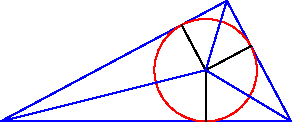
\includegraphics{china-inscribed}
\end{minipage}\medbreak
Here is a modern explanation. Given $a=8$ and $b=5$, the hypotenuse is $c=\sqrt{8^2+15^2}=17$, and the area of the large triangle is the sum of three smaller triangles, each having height $\frac 12 d$:
\[
	\frac 12 ab=\frac 12a\cdot\frac 12d+\frac 12b\cdot \frac 12d+\frac 12c\cdot\frac 12d
	\implies d=\frac{2ab}{a+b+c}
\]
Again we ask: is this a general method or an example?

\goodbreak






\begin{minipage}[t]{0.64\linewidth}\vspace{0pt}
	\boldinline{The Bamboo Problem}
	Here is another problem from the \emph{Nine Chapters}, as depicted in Yang Hui's 1262 \emph{Analysis of the Nine Chapters}.\smallbreak
	
	A bamboo has height 10 \emph{chi.} It breaks and the top touches the ground 3 \emph{chi} from the base of the stem. What is the height of the break?\smallbreak
	
	In modern language: if $a,b,c$ are the sides of the triangle with hypotenuse $c$, we know $\textcolor{Green}{b+c=10}$ and $\textcolor{blue}{a=3}$; we want $b$. The solution given is
	\[
		b=\frac 12\left(\textcolor{Green}{10}-\frac{\textcolor{blue}{3}^2}{\textcolor{Green}{10}}\right)=\frac{91}{20}\text{ \emph{chi}}
	\]
	Think about why!
\end{minipage}
\hfill
\begin{minipage}[t]{0.33\linewidth}\vspace{0pt}
	\flushright\includegraphics[scale=1]{bamboo-small}
\end{minipage}



\begin{minipage}[t]{0.64\linewidth}\vspace{0pt}
\boldinline{The Out-In Principle}

Liu made many other contributions to mathematics, including estimating $\pi$ in a manner similar to Archimedes. He made particular use of the \emph{out-in principle} for comparing area and volume:\medskip

\begin{enumerate}\itemsep0pt
  \item Area and volume are invariant under translations.
  \item If a figure is subdivided, the sum of the areas/volumes of the parts equals that of the whole.
\end{enumerate}
These are essentially axioms for area/volume in Euclidean geometry. For instance, Liu gave the argument shown in the picture in justification of the \emph{gao gu}: the large square is subdivided and the \emph{in} pieces $\textcolor{Green}{A_i,B_i,C_i}$ translated to new \emph{out} pieces $\textcolor{red}{A_o,B_o},\textcolor{blue}{C_o}$ to assemble the required squares.
\end{minipage}
\hfill
\begin{minipage}[t]{0.33\linewidth}\vspace{0pt}
	\flushright\includegraphics[scale=0.95]{outin}
\end{minipage}\medbreak

Liu extended the out-in principle to analyze solids, comparing the volumes of four basic solids:\par
\begin{minipage}[t]{0.4\linewidth}\vspace{0pt}
	\begin{itemize}
	  \item Cube (\emph{lifang})
	  \item Right triangular prism (\emph{qiandu})
	  \item Rectangular pyramid (\emph{yangma})
	  \item Tetrahedron (\emph{bienuan})
	\end{itemize}
\end{minipage}
\hfill
\begin{minipage}[t]{0.59\linewidth}\vspace{0pt}
	\flushright\includegraphics[scale=1]{fund-pieces-small}
\end{minipage}\medbreak
These could be assembled to calculate the volume of, say, a truncated pyramid:
\begin{center}
	\includegraphics[scale=1]{pyramid-small}
\end{center}
\goodbreak




\boldsubsection{Chinese Enumeration}

The ancient Chinese had two parallel systems of enumeration. Both are essentially decimal.

\boldinline{Oracle Bone Script and Modern Numerals}
  
The earliest Chinese writing, \emph{oracle bone} script, dates from around 1600\BC. The numbers 1--10 had distinct symbols, as did 20, 100, 1000 and 10000. These were decorated to denote various multiples. Some examples are shown below. 
\begin{center}
	\includegraphics[angle=1.4]{OracleBones-small.png}
  \includegraphics[angle=1.5]{OracleBones2-small.png}
\end{center}
Given all the possibilities for decoration, the system is complex and more advanced than other contemporary systems. Modern Chinese numerals are a direct descendant of this script:
\begin{center}
  \includegraphics[angle=-1.5]{ModernChinese-small.png}
  \includegraphics[angle=-1.5]{824ModernChinese-small.png}
\end{center}
Observe the similarity between the expressions for the first 10 digits. The second image denotes 842, where the second and fourth symbols represent 100's and 10's respectively (literally \emph{eight hundred four ten two}). A zero symbol is not required as a separator: one could not confuse 205 (\emph{two hundred five}) with 250 (\emph{two hundred five ten}). The system is partly positional: for instance the symbol for 8 can also mean 800 if placed correctly, but only if followed by the symbol for 100.


\boldinline{Rod Numerals and the Counting Board}
  
The second dominant form of enumeration dates from around 300\BC{} and was in wide use by \AD 300. Numbers were denoted by patterns known as \emph{zongs} and \emph{hengs}: \emph{zongs} represent units, 100's, 10000's, etc., while \emph{hengs} were for 10's, 1000's, 100000's, etc.
\begin{center}
  \includegraphics[angle=0.8]{ZongHeng-small.png}
\end{center}
Rod numerals were immensely practical---in extremis they could easily be scratched in the dirt! More commonly, short bamboo sticks or \emph{counting rods}---of which any merchant would carry a bundle---would be used in conjunction with a \emph{counting board}: a grid of squares on which sticks could be placed for ease of calculation. This technology facilitated easy trade and gave rise to several methods of calculation which will seem familiar. There was no need for a zero in this system as an empty space did the job. Variations of the rod numeral system persisted in China morphing into the \href{http://en.wikipedia.org/wiki/Suzhou_numerals}{\emph{Suzhou} system} which can still be found in some traditional settings.
\goodbreak


\boldinline{Basic Counting Board Calculations}

Addition and subtraction are straightforward by carrying and borrowing in the usual way. The smallest number was typically placed on the right. Multiplication is a little more fun. Here we multiply 387 by 147.
\begin{quote}
  \begin{tabular}{@{}l@{\qquad}l}
	  \begin{tabular}{|c|c|c|}
		  \hline
		  3&8&7\\\hline
		  &&\\\hline
		  1&4&7\\\hline
	  \end{tabular}
		&
		Arrange rods: we use modern numerals for clarity
		\\
		\\[-5pt]
  	\begin{tabular}{|c|c|c|c|c|}
		  \hline
		  &&3&8&7\\\hline
		  4&4&1&&\\\hline
		  1&4&7&&\\\hline
  	\end{tabular}
		&
		$3\times 147=441$, note the position of 147
		\\
		\\[-5pt]
	  \begin{tabular}{|c|c|c|c|c|}
		  \hline
		  &&&8&7\\\hline
		  4&4&1&&\\\hline
		  1&1&7&6&\\\hline
		  &1&4&7&\\\hline
	  \end{tabular}
		&
		Delete 3, move 147 and multiply: $8\times 147=1176$
		\\
		\\[-5pt]
	  \begin{tabular}{|c|c|c|c|c|}
		  \hline
		  &&&8&7\\\hline
		  5&5&8&6&\\\hline
		  &&&&\\\hline
		  &1&4&7&\\\hline
	  \end{tabular}
		&
		Sum rows
		\\
		\\[-5pt]
	  \begin{tabular}{|c|c|c|c|c|}
		  \hline
		  &&&&7\\\hline
		  5&5&8&6&\\\hline
		  &1&0&2&9\\\hline
		  &&1&4&7\\\hline
	  \end{tabular}
		&
		Delete 8, move 147 and multiply: $7\times 147=1029$
		\\
		\\[-5pt]
	  \begin{tabular}{|c|c|c|c|c|}
		  \hline
		  &&&&\\\hline
		  5&6&8&8&9\\\hline
		  &&1&4&7\\\hline
	  \end{tabular}
		&
		Sum rows: in conclusion, $387\times 147=56889$
  \end{tabular}
\end{quote}
The algorithm is just long-multiplication, starting with the largest digit (3) instead of the units as is more typical in Western education.\smallbreak
  
Division is similar to long-division. To divide 56889 by 147 one might have the following sequence of boards
\begin{quote}
  \begin{tabular}{|c|c|c|c|c|}
	  \hline
	  &&&&\\\hline
	  5&6&8&8&9\\\hline
	  &&1&4&7\\\hline
  \end{tabular} 
 	$\longrightarrow$
  \begin{tabular}{|c|c|c|c|c|}
	  \hline
	  &&3&&\\\hline
	  5&6&8&8&9\\\hline
	  1&4&7&&\\\hline
  \end{tabular}
  $\longrightarrow$
  \begin{tabular}{|c|c|c|c|c|}
	  \hline
	  &&3&8&\\\hline
	  1&2&7&8&9\\\hline
	  &1&4&7&\\\hline
  \end{tabular}
  $\longrightarrow$
  \begin{tabular}{|c|c|c|c|c|}
	  \hline
	  &&3&8&7\\\hline
	  &1&0&2&9\\\hline
	  &&1&4&7\\\hline
  \end{tabular}
\end{quote}
In the first two boards, 147 goes 3 times into 568.\par
In board 3, we subtract $3\times 147$ from 568 to leave 127, shift 147 one place to the right, and observe that 147 goes 8 times into 1278.\par
In the final step we have subtracted $8\times 147$ from 1278 to leave 102, before shifting 147 to its final position on the right. Since 147 divides exactly seven times into 1029, we are done.\smallbreak
There is nothing stopping us from dividing when the result is not an integer; one simply continues as in long-division, with fractions represented as decimals.
\goodbreak


\boldinline{Simultaneous linear equations}

The coefficients of a linear system were placed in adjacent \emph{columns} and then \emph{column operations} were performed. The method is identical to what you learn in a linear algebra class, but with columns rather than rows. Here is an example.
\[
	\begin{cases}
		3x+2y=7\\
		2x+y=4
	\end{cases}
	\longrightarrow\ 
	\begin{array}{|c|c|c|c|c|}
	  \hline
	  3&2\\\hline
	  2&1\\\hline
	  7&4\\\hline
  \end{array}
  \ \longrightarrow\ 
	\begin{array}{|c|c|c|c|c|}
	  \hline
	  1&2\\\hline
	  1&1\\\hline
	  3&4\\\hline
  \end{array}
  \ \longrightarrow\ 
	\begin{array}{|c|c|c|c|c|}
	  \hline
	  1&1\\\hline
	  1&0\\\hline
	  3&1\\\hline
  \end{array}
  \ \longrightarrow\ 
	\begin{array}{|c|c|c|c|c|}
	  \hline
	  0&1\\\hline
	  1&0\\\hline
	  2&1\\\hline
  \end{array}
  \ \longrightarrow x=1,\ y=2
\]
This matrix method was essentially unique to East Asia until the 1800s.


\boldinline{Euclidean algorithm}

The counting board lent also itself to the computation of greatest common divisors, which were used for simplifying fractions. Here is the process applied to $\frac{35}{91}$:
\[
	\begin{array}{llllllll}
		35&35&35&14&14&7\\
		91&56&21&21&7&7
	\end{array}
\]
At each stage, one subtracts the smaller number from the larger. Once the same number is in each row you stop. You should recognize the division algorithm at work! Since $\gcd(35,91)=7$, both could be divided by 7 to obtain $\frac{35}{91}=\frac 5{13}$ in lowest terms.


\boldinline{Negative numbers}

There is a strong case that the Chinese are the oldest adopters of negative numbers, though these were not originally thought of as such. Different colored rods were used to denote a deficiency in a quantity, commonly  when balancing accounts. The \emph{Nine Chapters} describes using red and black rods in this manner. This practice was known by \AD{1}, roughly 500 years before negative numbers were used in calculations in India. It is possible that there was some transference of this idea from China to India.
\smallskip


\begin{minipage}[t]{0.78\linewidth}\vspace{0pt}
	\boldinline{Music, Mysticism and Approximations} Like the Pythagoreans, the ancient Chinese were interested in music and pattern for mystical reasons. While the Pythagoreans delighted in the pentagram, the Chinese created \emph{magic squares} (grids whose rows, columns and diagonals sum to the same total) as symbols of perfection.
\end{minipage}
\hfill
\begin{minipage}[t]{0.2\linewidth}\vspace{0pt}
	\centering
	\begin{tabular}{|c|c|c|}
		\hline
		8&3&4\\\hline
		1&5&9\\\hline
		6&7&2\\\hline
	\end{tabular}
	\\[5pt]
	$3\times 3$ magic square
\end{minipage}\smallbreak

The notion of equal temperament in musical tuning was first `solved' in China by Zhu Zaiyu (1536--1611), some 30 years before Mersenne \& Stevin established the same idea in Europe. This required the computation of the twelfth-root of 2 which Zhu found using approximations for square and cube roots:
\[
	\sqrt[12]{2}=\sqrt[3]{\sqrt{\sqrt 2}}
\]
Zhu's approximation was correct to 24 decimal places! Indeed the Chinese emphasis on practicality meant that they often had the most accurate mathematical approximations of their time:
\begin{itemize}
  \item Approximations to $\pi$ including $\frac{22}7,\sqrt{10},\frac{355}{113},\frac{377}{120}$. Most accurate in the world from 400--1400.
  \item Methods for approximating square and cube roots were found earlier than in Europe. Approximations to solutions of higher-order equations similar to the Horner--Ruffini/Newton--Raphson method were also discovered earlier.
  \item Pascal's triangle first appeared in China around 1100. It later appeared in Islamic mathematics before making its way to Europe.
\end{itemize}

\goodbreak


\boldsubsubsection{Two Famous Problems}

We finish with two famous Chinese problems. The first is known as the  \emph{Hundred Fowl Problem} and dates from the 5\th{} century \AD\!. It was copied later in India and then by Leonardo da Pisa (Fibonacci) in Europe, thus demonstrating how some Chinese mathematics travelled westwards.

\begin{quote}
	If cockerels cost 5 \emph{qian } (a copper coin), hens 3 \emph{qian,} and 3 chicks cost 1 \emph{qian,} and if 100 fowl are bought for 100 \emph{qian,} how many cockerels, hens and chicks are there?
\end{quote}

In modern language, we want non-negative integers $x,y,z$ satisfying
\[
	\begin{cases}
	  5x+3y+\frac 13z=100\\
	  x+y+z=100
  \end{cases}
\]
The stated answers are $(4,18,78)$, $(8,11,81)$, $(12,4,84)$ while the solution $(0,25,75)$ was ignored.
\bigbreak

  
Finally we consider the \emph{Chinese Remainder Theorem} for solving simultaneous congruence equations. This result dates from the 4\th{} century \AD\!, after which it travelled to India where it was described by Bhramagupta, and thence to Europe. This example comes from Qin Jiushao's \emph{Shu Shu Jiu Zhang} (Nine Sections of Mathematics, 1247).  

\begin{quote}
	Three thieves stole three identical vessels filled with rice, but whose exact capacity was unknown. The thieves were caught and their vessels examined: the quantities left in each vessel were 1 \emph{ge,} 14 \emph{ge} and 1 \emph{ge} respectively. The thieves did not know the exact quantities they'd stolen. The first used a horse ladle (capacity 19 \emph{ge}) to take rice from the first vessel. The second used a wooden shoe (17 \emph{ge}) to take rice from his vessel. The third used a bowl (12 \emph{ge}). What was the total amount of rice stolen?
\end{quote}
  
In modern language, the capacity $x$ of each vessel satisfies
\[
	x\equiv 1\pmod{19},\qquad x\equiv 14\pmod{17},\qquad x\equiv 1\pmod{12}
\]
The given answer, $x=3193$ \emph{ge,} represents the smallest possible capacity of each vessel, with all other solutions being congruent modulo $19\cdot 17\cdot 12=3876$, as you should be able to confirm if you've studied number theory! The total amount of rice stolen is then
\[
	(x-1)+(x-14)+(x-1)=3x-16=9563
\]
Since congruence equations are simply underdetermined linear equations
\[
	x\equiv 1\pmod{19}\iff \exists y\in\Z\text{ such that }x=1+19y
\]
solutions to both of these problems can be effected using counting board methods.
  
\clearpage

  
\begin{exercisessec}{}{}
	\exstart Verify the result of the \emph{Bamboo problem.}
	
	\begin{enumerate}\setcounter{enumi}{1}
	  \item Solve the \emph{Hundred Fowl Problem} by substituting $z=100-x-y$ in the first equation and observing that $x$ must be divisible by 4.
	% 
	%     As a possible method, one substitutes $z=100-x-y$ in first equation to obtain $7x+4y=100$, or
	%   \[y=25-\frac 74x\]
	%   Since $y\in\Z$, we must have $x=4m$ for some integer $m$. Thus all solutions have the form
	%   \[x=4m,\quad y=25-7m,\quad z=75+3m,\quad m\in\Z\]
	%   For $m=1,2,3$ and 0 we obtain the above solutions. For $m\ge 4$ we have $y<0$, while $m<0$ yields $x<0$.
	
		\item Use a counting board method to:
		\begin{enumerate}
		  \item Solve the linear system
		  $\begin{cases}
		  	8x+y=28\\
		  	3x+2y=17
		  \end{cases}$
			\item Multiply $218\times 191$.
		\end{enumerate}
		
	
	  
	  \begin{minipage}[t]{0.53\linewidth}\vspace{0pt}
		  \item\label{exs:gaoguproof}%[7-10]
		  Turn Zhao Shuang's pictorial argument from the \emph{Arithmetical Classic of the Gnomon} into a proof of Pythagoras' Theorem.
	 	\end{minipage}
	 	\hfill
	 	\begin{minipage}[t]{0.46\linewidth}\vspace{0pt}
	 		\flushright\includegraphics[scale=0.25,angle=-1]{ZhaoPythag}
	  \end{minipage}
	
	
	% 	\item%[7-4]
	% 	Look up the description of the \emph{Woman Weaving} problem from the \emph{Suanshu shu} and solve it using the method described in the textbook.
		
		\item Solve problem 24 of chapter 9 of  the \emph{Nine Chapters.}
		\begin{quote}
			A deep well 5 ft in diameter is of unknown depth (to the water level). If a 5 ft post is erected at the edge of the well, the line of sight from the top of the post to the edge of the water passes through a point 0.4 ft from the lip of the well below the post. What is the depth of the well?
		\end{quote}
	  
	  \item%[7-6]
	  Solve problem 26 of chapter 6 of the \emph{Nine Chapters.}
	  \begin{quote}
	  	Five channels bring water into a reservoir. If only the first channel is open, the reservoir fills in $\frac 13$ of a day. The second channel by itself fills the reservoir in 1 day, the third channel in $2\frac 12$ days, the fourth in 3 days, and the fifth in 5 days. If all the channels are opened together, how long will the reservoir take to fill?
	  \end{quote}
	
	\end{enumerate}  

\end{exercisessec}